% Part: sets-functions-relations
% Chapter: relations
% Section: graphs

\documentclass[../../../include/open-logic-section]{subfiles}

\begin{document}

\olfileid{sfr}{rel}{grp}
\olsection{گراف}

\emph{گراف} اک خاکہ اے جیہدے وچ نقطے---جنہاں نوں «گرہاں» یا «راس»
(اک لئی وی «راس») آکھدے نیں---کناریاں نال جڑے ہوندے نیں۔ گراف گسستہ
ریاضی تے کمپیوٹر سائنس وچ تھاں تھاں ورتے جان والے اوزار نیں۔ ایہ
تعلقاں تے بناوٹاں دی نمائندگی کرن تے اوہناں نوں اکھاں اگے لیاؤن لئی
بہت کم آؤندے نیں؛ مختلف قسماں دے نیٹ ورکاں ورگیاں ٹھوس چیزاں توں لے کے
فیصلیاں دے ممکنہ نتیجیاں ورگیاں مجرد بناوٹاں تیکر۔ علمی لکھتاں وچ
گرافاں دیاں بہت وکھ وکھ قسماں ملدیاں نیں۔ اوہ، مثال دے طور تے، ایہناں
گلاں وچ وکھریاں ہوندیاں نیں کہ کناریاں دی سمت اے یا نہیں، اوہناں اُتے
لیبل نیں یا نہیں، کسے گرہ توں اوسے گرہ ول کنارا ہو سکدا اے یا نہیں،
اوہناں ای گرہاں دے وچکار اک توں ودھ کنارے ہو سکدے نیں یا نہیں، وغیرہ۔
\emph{سمت دار گرافاں} دا تعلقاں نال خاص جوڑ اے۔

\begin{defn}[سمت دار گراف]
اک \emph{سمت دار گراف} $G = \tuple{V, E}$، \emph{راساں} دے اک سیٹ~$V$
تے \emph{کناریاں} دے اک سیٹ~$E \subseteq V^2$ توں بندا اے۔
\end{defn}

\begin{explain}
ساڈی تعریف مطابق، گراف بس اک سیٹ تے اوس سیٹ اُتے اک تعلق اے۔ بے شک،
جدوں گرافاں دی گل کریے، تاں ایہ توقع فطری اے کہ اوہناں نوں خاکے دی
صورت وچ وکھایا جاوے: اسی دو راساں~$v_1$ تے $v_2$ نوں تیر نال اُدوں
تے صرف اُدوں جوڑ کے گراف بنا سکدے آں جدوں $\tuple{v_1, v_2} \in E$۔
اپنے آپ وچ اک تعلق تے اک گراف وچ فرق صرف ایہ اے کہ گراف راساں دا
سیٹ وی دسدا اے، یعنی گراف وچ الگ تھلگ راس وی ہو سکدے نیں۔ پر اہم گل
ایہ اے کہ ہر تعلق~$R$ جیہڑا کسے سیٹ~$X$ اُتے ہووے، سمت دار گراف
$\tuple{X, R}$ دے طور تے ویکھیا جا سکدا اے؛ تے اُلٹ پاسے، سمت دار
گراف~$\tuple{V, E}$ نوں تعلق $E \subseteq V^2$ دے طور تے ویکھیا جا سکدا
اے، جیہدے نال سیٹ $V$ صاف طور تے دسیا ہووے۔
\end{explain}

\begin{ex}
گراف $\tuple{V, E}$، جیہدے لئی $V = \{1, 2, 3, 4\}$ تے $E =
\{\tuple{1,1}, \allowbreak \tuple{1, 2}, \allowbreak \tuple{1, 3},
\allowbreak \tuple{2, 3}\}$، ایویں دکھائی دیندا اے:
\begin{align*}
& 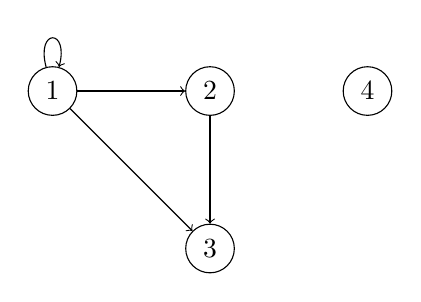
\begin{tikzpicture}[->,node distance=2cm]
  \node[draw,circle] (A) {$1$};
  \node[draw,circle] (B) [right of=A] {$2$};
  \node[draw,circle] (C) [below of=B] {$3$};
  \node[draw,circle] (D) [right of=B] {$4$};
  \draw (A) to [loop above]  (A);
  \draw (A) to  (B);
  \draw (A) to  (C);
  \draw (B) to  (C);
  \end{tikzpicture}
\intertext{ایہ گراف، گراف $\tuple{V', E}$ توں وکھرا اے جیہدے لئی $V' =
  \{1, 2, 3\}$؛ اوہ ایویں دکھائی دیندا اے:}
& 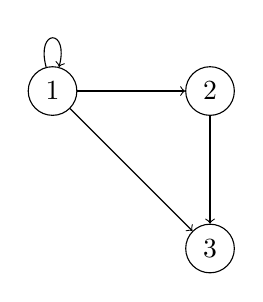
\begin{tikzpicture}[->,node distance=2cm]
  \node[draw,circle] (A) {$1$};
  \node[draw,circle] (B) [right of=A] {$2$};
  \node[draw,circle] (C) [below of=B] {$3$};
  \draw (A) to [loop above]  (A);
  \draw (A) to  (B);
  \draw (A) to  (C);
  \draw (B) to  (C);
  \end{tikzpicture}
\end{align*}
\end{ex}

\begin{prob}
  گھٹ یا برابر ہون دے تعلق~$\le$ نوں، سیٹ $\{1, 2, 3, 4\}$ اُتے، گراف
  دے طور تے ویکھو تے اوہدا خاکہ بناؤ۔
\end{prob}

\end{document}
